\documentclass[preview]{standalone}
\usepackage{tikz}
\usetikzlibrary{automata, arrows.meta}
\begin{document}
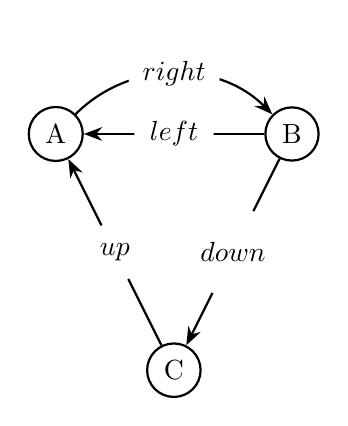
\begin{tikzpicture}
\begin{scope}[every node/.style={circle,thick,draw}]
    \node (A) at (0,0)    {A};
    \node (B) at (3,0)    {B};
    \node (C) at (1.5,-3) {C};
\end{scope}

\begin{scope}[>={Stealth[black]},
            every node/.style={fill=white,circle},
            every edge/.style={draw=black,thick}]
    \path [->] (A) edge [bend left=45] node {$right$} (B);
    \path [->] (B) edge node [bend pos=-2] {$left$}  (A);
    \path [->] (B) edge node {$down$}  (C);
    \path [->] (C) edge node {$up$}    (A);
\end{scope}
\end{tikzpicture}
\end{document}
